\section{Deep Q-learning}

\subsection{Q-сетка}

В сложных средах пространство состояний может быть непрерывно или конечно, но велико (например, пространство всех экранов видеоигры). В таких средах моделировать функции от состояний, будь то стратегии или оценочные функции, мы можем только приближённо при помощи параметрических семейств.

\needspace{7\baselineskip}
\begin{wrapfigure}{r}{0.35\textwidth}
\vspace{-0.3cm}
\centering
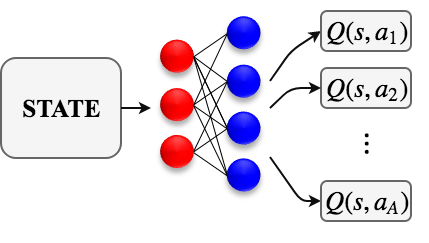
\includegraphics[width=0.3\textwidth]{Images/Qnetwork2.png}
\vspace{-0.3cm}
\end{wrapfigure}

Далее мы будем предполагать, что Q-функция задана нейросеткой $Q^*(s, a, \theta)$ с параметрами $\theta$. Заметим, что для дискретных пространств действий сетка может как принимать действия на входе, так и принимать на вход только состояние $s$, а выдавать $|\A|$ чисел $Q^*(s, a_1, \theta) \dots Q^*(s, a_{|\A|}, \theta)$. В последнем случае мы можем за константу находить жадное действие $\pi(s) = \argmax\limits_a Q^*(s, a, \theta)$.

В случае, если пространство действий непрерывно, выдать по числу для каждого варианта уже не получится. При этом, если непрерывное действие подаётся на вход вместе с состоянием, то оптимизировать по нему для поиска максимума или аргмаксимума придётся при помощи серии прямых и обратных проходов (для дискретного пространства --- за $|\A|$ прямых проходов), что вычислительно ни в какие ворота. Поэтому такой вариант на практике не встречается, а алгоритм пригоден в таком виде только для дискретных пространств состояний (позже мы пофиксим это при обсуждении алгоритма DDPG, раздел \ref{DDPGsection}).

\begin{remark}
Использование нейросеток позволяет обучаться для сред, в которых состояния $s$ заданы, например, пиксельным представлением экранов видеоигр. Стандартным вариантом архитектуры является несколько (не очень много) свёрточных слоёв, обычно без использования макспулингов (важно не убить информацию о расположении распознанных объектов на экране). Использование батч-нормализаций и дроп-аутов сопряжено с вопросами о том, нужно ли их включать-выключать на этапах генерации таргетов (который, как мы увидим позже, тоже распадается на два этапа), сборе опыта с возможностью исследования и так далее. Чаще их не используют, чем используют, так как можно нарваться на неожиданные эффекты. Важно помнить, что все эти блоки были придуманы для решения немного других задач, и стоит осторожно переносить их в контекст обучения с подкреплением.
\end{remark}

\subsection{Переход к параметрической Q-функции}\label{toregression}

Итак, мы хотим адаптировать алгоритм Q-learning для случая, когда оптимальная Q-функция представлена дифференцируемой по параметрам $\theta$ функцией $Q^*(s, a, \theta)$. 

Вообще говоря, мы помним, что мы хотим решать уравнения оптимальности Беллмана \eqref{Q*Q*}, и можно было бы, например, оптимизировать невязку:
$$\left( Q^*(s, a, \theta) - r(s, a) - \gamma \E_{s'} \max_{a'} Q^*(s', a', \theta) \right)^2 \to \min_{\theta}$$
однако мат.ожидание $\E_{s'}$ в формуле берётся по неизвестному нам распределению (а даже если известному, то почти наверняка в сложных средах аналитически ничего не возьмётся) и никак не выносится (несмещённые оценки градиента нас бы устроили).

В Q-learning-е мы смогли с сохранением теоретических гарантий побороться с этим при помощи стохастической аппроксимации, получив формулу \eqref{Qlearningupdate}. Хочется сделать какой-то аналогичный трюк:
$$Q^*(s, a, \theta) \leftarrow Q^*(s, a, \theta) + (1 - \alpha)\left( r(s, a) + \gamma \max_{a'} Q^*(s', a', \theta) - Q^*(s, a, \theta) \right)$$

Мы уже отмечали ключевое наблюдение о том, что формула стохастической аппроксимации очень напоминает градиентный спуск, а $\alpha$ играет роль learning rate. Да даже условия сходимости \ref{TDconvergence}, собственно, те же, что в стохастическом градиентном спуске\footnote{это не случайность: корни теории одни и те же.}! И, действительно, табличный Q-learning является градиентным спуском для решения некоторой задачи регрессии.

Поскольку это очень принципиальный момент, остановимся в этом месте подробнее. Пусть у нас есть текущая версия $Q^*(s, a, \theta_k)$, и мы хотим проделать шаг метода простой итерации для решения уравнения Q*Q* \eqref{Q*Q*}. Зададим следующую задачу регрессии:
\begin{itemize}
\item входом является пара $s, a$
\item искомомым (!) значением на паре $s, a$ --- правая часть уравнения оптимальности Беллмана \eqref{Q*Q*}, т.е.
$$f(s, a) \coloneqq r(s, a) + \gamma \E_{s'} \max_{a'} Q^*(s', a', \theta_k) $$
\item наблюдаемым (<<зашумлённым>>) значением целевой переменной или \emph{таргетом} (target)
\begin{equation}\label{guess}
y(s, a) \coloneqq r(s, a) + \gamma \max_{a'} Q^*(s', a', \theta_k)
\end{equation}
где $s' \sim p(s' \mid s, a)$
\item функцией потерь MSE:
$\Loss(y, \hat{y}) = \frac{1}{2}(y - \hat{y})^2$
\end{itemize}

Заметим, что, как и в классической постановке задачи машинного обучения, значение целевой переменной --- это её <<зашумлённое>> значение: по входу $s, a$ генерируется $s'$, затем от $s'$ считается детерминированная функция, и результат $y$ является наблюдаемым значением. Мы можем для данной пары $s, a$ засэмплировать себе таргет, взяв переход $(s, a, r, s')$ и воспользовавшись сэмплом $s'$, но существенно, что такой таргет --- случайная функция от входа. Принципиально: согласно уравнениям Беллмана, мы хотим выучить мат.ожидание такого таргета, а значит, нам нужна квадратичная функция потерь.

\begin{theorem}
Пусть $Q^*(s, a, \theta_{k+1})$ --- достаточно ёмкая модель (model with enough capacity), выборка неограниченно большая, а оптимизатор идеальный. Тогда решением вышеописанной задачи регрессии будет шаг метода простой итерации для поиска оптимальной Q-функции:
$$Q^*(s, a, \theta_{k+1}) = r(s, a) + \gamma \E_{s'} \max_{a'} Q^*(s', a', \theta_k)$$
\beginproof
Под <<достаточно ёмкой моделью>> подразумевается, что модель может имитировать любую функцию, например для каждой пары $s, a$ из выборки выдавать любое значение. Найдём оптимальное значение для пары $s, a$: для неё $Q^*(s, a, \theta_{k+1})$ выдаёт некоторое число, которое должно минимизировать MSE:
$$\frac{1}{2}\E_{s'} \left( y(s, a) - Q^*(s, a, \theta_{k+1}) \right)^2 \to \min_{\theta_{k+1}}$$
Оптимальным константным решением регрессии с MSE как раз является среднее, получаем
\begin{align*}
    Q^*(s, a, \theta_{k+1}) = \E_{s'} y(s, a) = r(s, a) + \gamma \E_{s'} \max_{a'} Q^*(s', a', \theta_k) \tagqed
\end{align*}
\end{theorem}

В частности, формула Q-learning \eqref{Qlearningupdate} --- это частный случай решения указанной задачи регрессии стохастическим градиентным спуском для специального вида параметрических распределений:

\begin{theorem}
Пусть Q-функция задана табличным параметрическим семейством, а то есть табличкой размера $|\St|$ на $|\A|$, где в каждой ячейке записан параметр $\theta_{s, a}$:
$$Q^*(s, a, \theta) = \theta_{s, a}$$
Тогда формула \eqref{Qlearningupdate} представляет собой градиентный спуск для решения обсуждаемой задачи регрессии.

\begin{proof}
Посчитаем градиент функции потерь на одном объекте $s, a$. Предсказанием модели будет $\hat{y} = Q^*(s, a, \theta) = \theta_{s, a}$, то есть градиент предсказания по параметрам модели равен
$$\nabla_\theta \hat{y} = e_{s, a}$$
где $e_{s, a}$ --- вектор из $\R^{|\St| |\A|}$ из всех нулей с единственной единичкой в позиции, соответствующей паре $s, a$. Теперь посчитаем градиент функции потерь:
$$\nabla_\theta \Loss \left( y, \hat{y}(\theta) \right) = \left( \hat{y} - y(s, a) \right) \nabla_\theta \hat{y} = \left( Q^*(s, a, \theta_t) - y(s, a) \right) e_{s, a}$$
Итак, градиентный спуск делает следующие апдейты параметров:
$$\theta_{k+1} = \theta_k - \alpha \nabla_\theta \Loss \left( y, \hat{y} \right) = \theta_k + \alpha \left( y(s, a) - Q^*(s, a, \theta_t) \right) e_{s, a}$$
В этой формуле обновляется ровно одна ячейка таблички $\theta_{s, a}$, и это в точности совпадает с \eqref{Qlearningupdate}.
\end{proof}
\end{theorem}

Принципиально важно, что зависимость целевой переменной $y(s, a)$ \eqref{guess} от параметров $\theta$ игнорируется. На одном шаге алгоритма мы хотим провести шаг метода простой итерации, но не можем взять мат.ожидание, и решаем эту проблему, составляя задачу регрессии, где $y$ --- зафиксированная целевая переменная. Если вдруг в неё протекует градиенты, мы будем не только подстраивать прошлое под будущее, но и будущее под прошлое, что не будет являться корректной процедурой.

Важно, что как только мы от <<табличных параметрических функций>> переходим к произвольным параметрическим семействам, все теоретические гарантии сходимости Q-learning-а \ref{TDconvergence} теряются (теоремы сходимости использовали <<табличность>> нашего представления Q-функции). Как только мы используем ограниченные параметрические семейства вроде нейросеток, неидеальные оптимизаторы вроде Адама или не доводим каждый этап метода простой итерации до сходимости, гарантий нет.

\subsection{Декорреляция сэмплов}

Q-learning после одного шага в среде делал апдейт одного значения таблицы $Q^*(s, a)$. Сейчас нас такой вариант, очевидно, не устраивает, потому что обучать нейросетки на мини-батчах размера 1 (особенно с уровнем доверия к нашим таргетам) --- это явно плохая идея, но главное, сэмплы $s, a, y$ сильно скоррелированы: в сложных средах последовательности состояний обычно очень сильно похожи. Нейросетки на скоррелированных данных обучаются очень плохо (чаще --- не обучаются вовсе). Поэтому сбор мини-батча подряд с одной траектории здесь не сгодится.

\begin{center}
    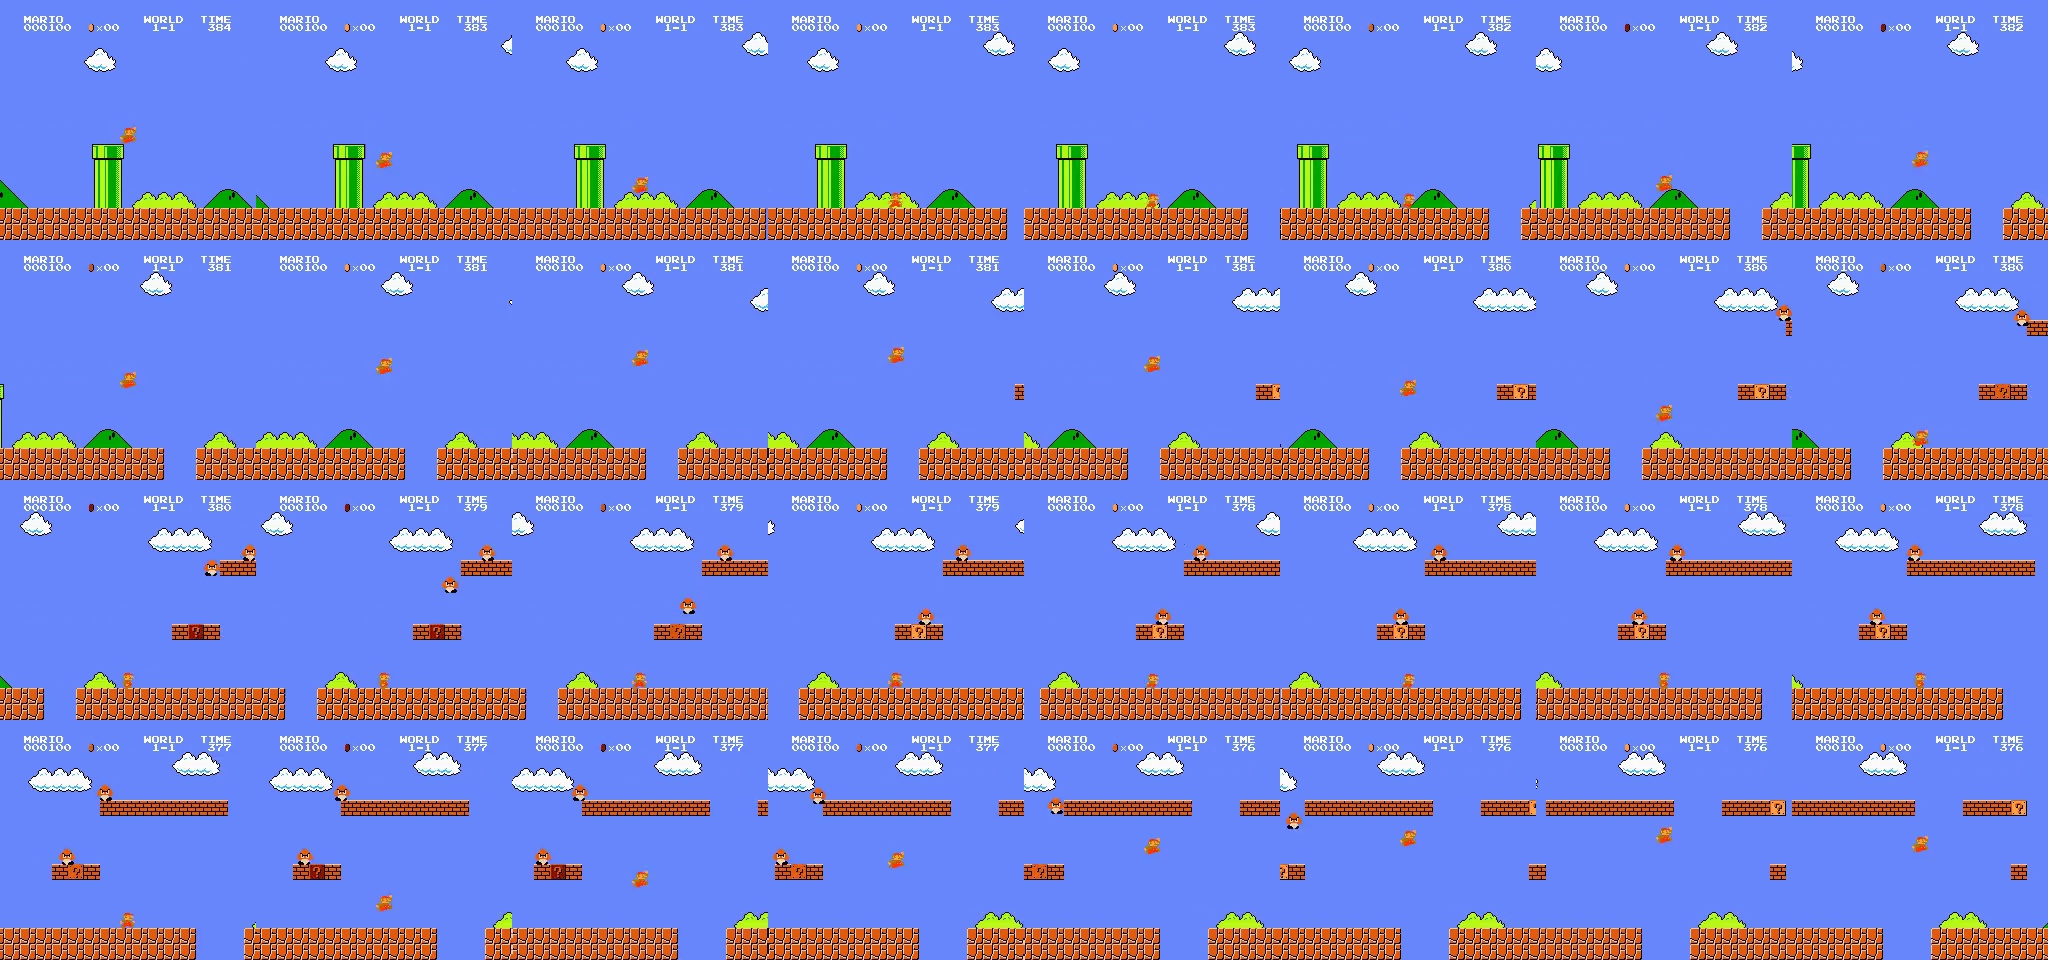
\includegraphics[width=\textwidth]{Images/correlated.jpg}
\end{center}

Есть два доступных на практике варианта \emph{декорреляции сэмплов} (sample decorrelation). Первый --- запуск параллельных агентов, то есть сбор данных сразу в нескольких параллельных средах. Этот вариант доступен всегда, по крайней мере, если среда виртуальна; иначе эта опция может быть дороговатой... Второй вариант --- реплей буфер, который, как мы помним, является прерогативой исключительно off-policy алгоритмов.

\begin{remark}
На практике картинки в какой-то момент начинают переполнять оперативку и начинаются проблемы. Простое решение заключается в том, чтобы удалять самые старые переходы, то есть оставлять самый новый опыт, однако есть альтернативные варианты (см. приоритизированный реплей, раздел \ref{subsec:prioritizedreplay})
\end{remark}

При наличии реплей буфера агент может решать задачи регрессии, сэмплируя мини-батчи переходов $\T \HM= (s, a, r', s')$ из буфера, затем делая для каждого перехода расчёт таргета $y(\T) \coloneqq r \HM+ \gamma \max\limits_{a'} Q^*(s', a', \theta)$, игнорируя зависимость таргета от параметров, и проводя шаг оптимизации по такому мини-батчу. Такой батч уже будет декоррелирован.

\begin{center}
    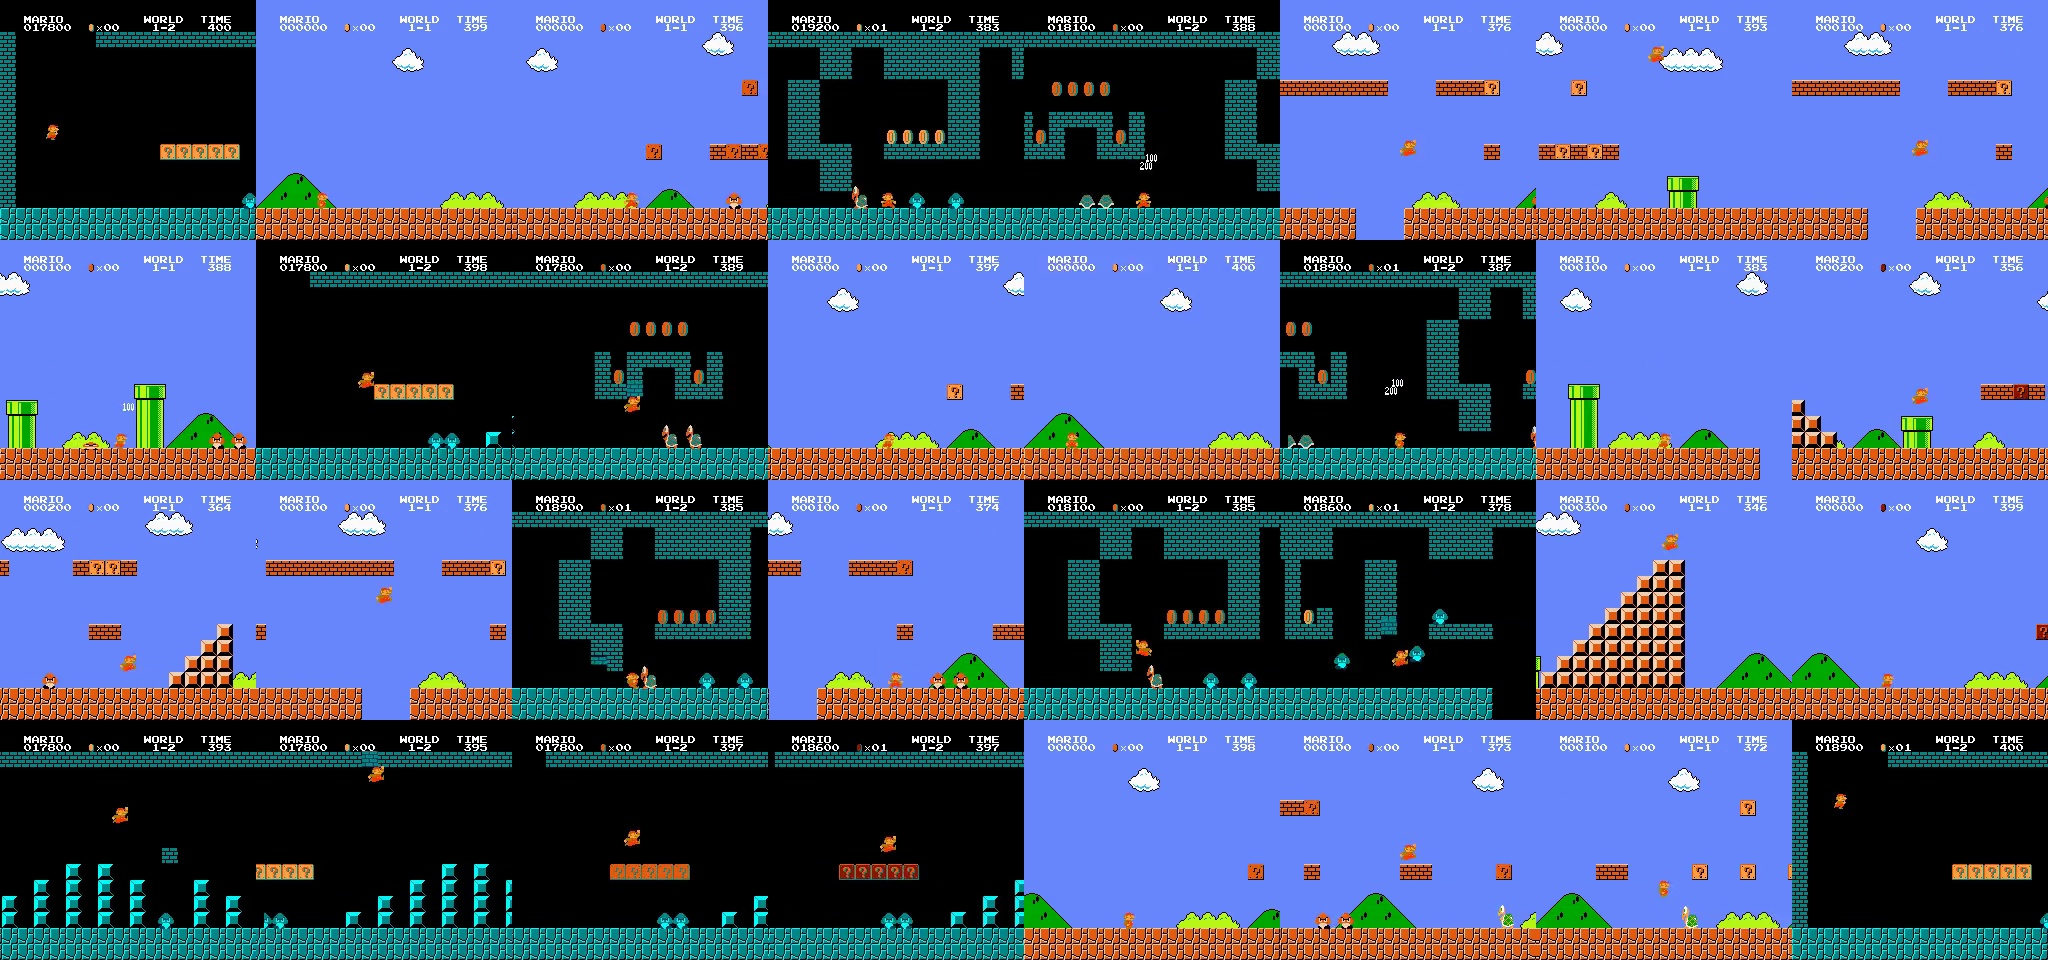
\includegraphics[width=\textwidth]{Images/decorrelated.jpg}
\end{center}

Почему мы можем использовать здесь реплей буфер? Если бы мы решали уравнения оптимальности Беллмана \eqref{Q*Q*} минимизацией невязки (каким-то образом вычисляя точное мат.ожидание по динамике среды), мы бы минимизировали какую-нибудь сумму невязок по всем парам $s, a$. Поэтому в поставленной задаче регрессии мы можем брать тройки $s, a, y$ для обучения из условно произвольного распределения до тех пор, пока оно достаточно разнообразно и нескоррелированно. Единственное ограничение --- внутри $y$ сидит $s'$, который должен приходить из и только из $p(s' \mid s, a)$. Но поскольку среда однородна, любые тройки $s, a, s'$ из любых траекторий, сгенерированных любой стратегией, таковы, что $s' \sim p(s' \mid s, a)$, а значит, $s'$ может быть использован для генерации таргета. Иными словами, в рамках текущего подхода мы, как и в табличном Q-learning-е, находимся в off-policy режиме, и наши условия на процесс порождения переходов $s, a, r, s'$ точно такие же.

\subsection{Таргет-сеть}

Концептуально, мы поняли, что на очередном шаге алгоритма нам нужно зафиксировать целевую переменную $y(s, a)$ по формуле \eqref{guess}, провести несколько итераций градиентного спуска, и затем переходить к следующему шагу метода простой итерации, на котором задача регрессии изменится (поменяется целевая переменная). Учитывая, что целевая переменная, которая во время решения задачи регрессии считается ground truth-ом, строится с использованием текущего приближения Q-функции, возникает естественное желание менять целевую переменную каждый шаг, то есть после каждого градиентного шага использовать новую версию Q-функции для генерации таргета. Эмпирически легко убедиться, что такой подход нестабилен примерно от слова совсем. 

Для стабилизации процесса одну задачу регрессии нужно решать более одной итерации градиентного спуска; необходимо сделать хотя бы условно 100-200 шагов. Проблема в том, что если таргет строится по формуле $r + \gamma \max\limits_{a'} Q^*(s, a, \theta)$, то после первого же градиентного шага $\theta$ поменяется.

\needspace{7\baselineskip}
\begin{wrapfigure}{r}{0.4\textwidth}
\vspace{-0.3cm}
\centering
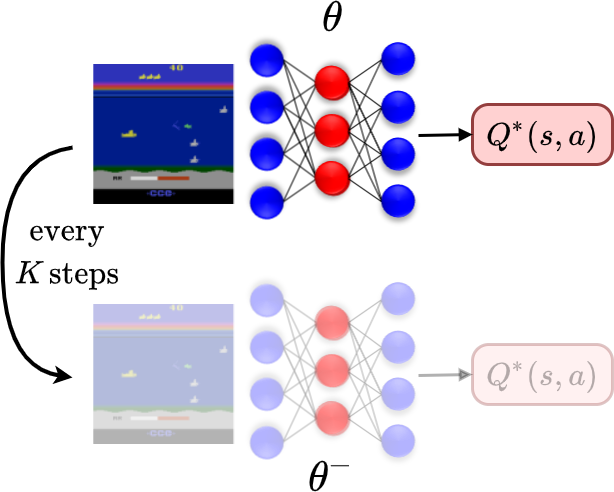
\includegraphics[width=0.4\textwidth]{Images/targetNetwork.png}
\vspace{-1.5cm}
\end{wrapfigure}

Вычисление таргета для всего реплей буфера, конечно же, непрактично: реплей буфер обычно огромен (порядка $10^6$ переходов), а одна задача регрессии будет решаться суммарно 100-200 шагов на мини-батчах размера, там, 32 (итого таргет понадобится считать всего для порядка 3000 переходов). Поэтому хранится копия $Q$-сетки, называемая \emph{таргет-сетью} (target network), единственная цель которой --- генерировать таргеты текущей задачи регрессии для транзишнов из засэмплированных мини-батчей. Будем обозначать её параметры как $\theta^{-}$. Итак, целевая переменная в таких обозначениях генерится по формуле
$$y( \T ) \coloneqq r + \gamma \max\limits_{a'} Q^*(s', a', \theta^{-})$$
а раз в $K$ шагов веса $\theta^{-}$ просто копируются из текущей модели с весами $\theta$ для <<задания>> новой задачи регрессии.

\begin{remark}
При обновлении задачи регрессии график функции потерь типично подскакивает. Поэтому распространённой, но чуть более вычислительно дорогой альтернативой является на каждом шаге устраивать экспоненциальное сглаживание весов таргет сети. Тогда на каждом шаге:
$$\theta^{-} \leftarrow (1 - \alpha) \theta^{-} + \alpha \theta,$$
где $\alpha$ --- гиперпараметр. Такой вариант тоже увеличивает стабильность алгоритма хотя бы потому, что решаемая задача регрессии меняется <<постепенно>>.
\end{remark}

\subsection{DQN}

Собираем алгоритм целиком. Нам придётся оставить $\eps$-жадную стратегию исследования --- с проблемой исследования-использования мы ничего пока не делали, и при стартовой инициализации есть риск отправиться тупить в ближайшую стену. Также лишний раз вспомним про то, что в терминальных состояниях обязательно нужно домножаться на $(1 - \done)$, поскольку шансов у приближённого динамического программирования сойтись куда-то без <<отправной точки>> не очень много. 

\begin{algorithm}[label = DQNalgorithm]{Deep Q-learning (DQN)}
\textbf{Гиперпараметры:} $B$ --- размер мини-батчей, $K$ --- периодичность апдейта таргет-сети, $\eps(t)$ --- стратегия исследования, $Q^*$ --- нейросетка с параметрами $\theta$, SGD-оптимизатор

\vspace{0.3cm}
Инициализировать $\theta$ произвольно \\
Положить $\theta^- \coloneqq \theta$ \\
Пронаблюдать $s_0$ \\
\textbf{На очередном шаге $t$:}
\begin{enumerate}
    \item выбрать $a_t$ случайно с вероятностью $\eps(t)$, иначе $a_t \coloneqq \argmax\limits_{a_t} Q^*(s_t, a_t, \theta)$
    \item пронаблюдать $r_t$,  $s_{t+1}$, $\done_{t+1}$
    \item добавить пятёрку $(s_t, a_t, r_t, s_{t+1}, \done_{t+1})$ в реплей буфер
    \item засэмплировать мини-батч размера $B$ из буфера
    \item для каждого перехода $\T = (s, a, r, s', \done)$ посчитать таргет:
    $$y(\T ) \coloneqq r + \gamma (1 - \done) \max\limits_{a'} Q^*(s', a', \theta^-)$$
    \item посчитать лосс:
    $$\Loss(\theta) \coloneqq \frac{1}{B}\sum_{\T} \left( Q^*(s, a, \theta) - y(\T ) \right) ^2$$
    \item делаем шаг градиентного спуска по $\theta$, используя $\nabla_\theta \Loss(\theta)$
    \item если $t \operatorname{mod} K = 0$: $\theta^- \gets \theta$
\end{enumerate}
\end{algorithm}